\documentclass[12pt]{report}

% Packages
\usepackage{acronym}
\usepackage{amsmath}
\usepackage{amsthm}
\usepackage{amsfonts}
\usepackage{epigraph}
\usepackage{geometry}
\usepackage{graphicx}
%\usepackage{mdframed}
\usepackage{titlesec}
\usepackage{caption}
\usepackage{listings}
\usepackage{xcolor}
\usepackage{siunitx}
\usepackage{enumitem}
\usepackage{pdfpages}
\usepackage[utf8]{inputenc}
\usepackage{fancyhdr}
\usepackage{transparent}
\usepackage[hidelinks, colorlinks=true, linkcolor=blue, urlcolor=blue, citecolor=blue]{hyperref}
\usepackage[backend=biber, style=ieee]{biblatex}
%\addbibresource{cdt_app.bib}

% Acronym set-up
% Command to insert acronyms with a temporary color change
\newcommand{\myAcro}[1]{{\hypersetup{linkcolor=black}\acl{#1}}} % For acronym list (full form)
\newcommand{\myAcroLink}[1]{{\hypersetup{linkcolor=black}\acs{#1}}}

% Document geometry setup
\geometry{
    a4paper,
    margin=2cm,
    top=1cm,    % Adjust top margin
    bottom=1cm,  % Adjust bottom margin
    headheight=14.5pt,
    includeheadfoot
}

\pagestyle{fancy} % Use fancy style for all pages
\fancyhf{} % Clear all header and footer fields

% Header
\fancyhead[L]{{\transparent{0.5}Chapter \udlchap{} Questions}} % Left header
\fancyhead[R]{{\transparent{0.5}wp289}} % Right header

% Footer
\fancyfoot[L]{\transparent{0.5}Understanding Deep Learning} % Left footer
\fancyfoot[R]{\transparent{0.5}\thepage} % Right footer

% Define line thickness
\renewcommand{\headrulewidth}{0.4pt}
\renewcommand{\footrulewidth}{0.4pt}

% Redefining plain page style if needed
\fancypagestyle{plain}{ % Applies to chapter beginnings and similar
  \fancyhf{} % clear all header and footer fields for plain style
  \renewcommand{\headrulewidth}{0.4pt}
  \renewcommand{\footrulewidth}{0.4pt}
  \fancyhead[L]{{\transparent{0.5}Chapter \udlchap{}Questions}}
  \fancyhead[R]{{\transparent{0.5}wp289}}
  \fancyfoot[L]{\transparent{0.5}Understanding Deep Learning}
  \fancyfoot[R]{\transparent{0.5}\thepage}
}

% Customise Chapter Headings
\titleformat{\chapter}
    {\normalfont\LARGE\bfseries}
    {\thechapter.}
    {1em}
    {}
\titlespacing*{\chapter}{0pt}{-20pt}{\baselineskip}

% Customise section spacing
\titlespacing*{\section}{0pt}{\baselineskip}{0.5\baselineskip}

% Adjusting space around figures
\setlength{\floatsep}{5pt}
\setlength{\textfloatsep}{5pt}

% Adjusting caption spacing
\captionsetup{aboveskip=5pt, belowskip=5pt}

% Format paragraphs
\setlength{\parindent}{0pt}
\setlength{\parskip}{1em}  % Adjust the value as needed

% Adjust list spacing
%\setlist[enumerate]{before=\vspace{0.5em}, after=\vspace{0.5em}}
\setlist[enumerate]{before=\vspace{-0.5\baselineskip}, after=\vspace{-0.5\baselineskip}}

% Customise question boxes
\usepackage[framemethod=TikZ]{mdframed}
\mdfsetup{
    backgroundcolor=gray!20,
    innertopmargin=10pt,
    innerbottommargin=10pt,
    skipbelow=0pt 
}

\def\udlchap{10}
\renewcommand{\thesubsection}{Problem \udlchap.\arabic{subsection}}

%%%%%%%%%%%%%%%%%%%%%%%%%%%%%%%%%%%%%%%%%%%%%%%%%%%%%%%%%

\begin{document}

\section*{Chapter 10: Convolutional networks}

\subsection{}
\begin{mdframed}
    Show that the operation in equation 10.4 is equivariant with respect to translation.
\end{mdframed}

\begin{equation}
    h_{i} = \text{a}[\beta + \omega_{1}x_{i-1} + \omega_{2}x_{i} + \omega_{3}x_{i+1}]
    \tag{10.4}
\end{equation}

A function is equivariant to a transformation $t(x)$ if $f(t(x)) = t(f(x))$. In this case, the transformation is translation, so $t(x) = x + \delta$. Let's denote the transformed sequence as $\{x_{i}'\}$ and the function as $h_{i}'$:

\begin{equation*}
    h_{i}' = \text{a}[\beta + \omega_{1}x_{i-1}' + \omega_{2}x_{i}' + \omega_{3}x_{i+1}']
\end{equation*}

Substitute $x_{i}' = x_{i} + \delta$:

\begin{equation*}
    h_{i+\delta} = \text{a}[\beta + \omega_{1}x_{i+ \delta-1} + \omega_{2}x_{i+ \delta} + \omega_{3}x_{i+ \delta+1}]
\end{equation*}

Which shows that $h_{i}' = h_{i+\delta}$, demonstrating that this operation is is equivariant with respect to translation by any integer $\delta$.


\subsection{}
\begin{mdframed}
    Equation 10.3 defines 1D convolution with a kernel size of three, stride of one, and dilation one. Write out the equivalent equation for the 1D convolution with a kernel size of three and a stride of two as pictured in figure 10.3a-b.
\end{mdframed}

\begin{equation}
    z_{i} = \omega_{1}x_{i-1} + \omega_{2}x_{i} + \omega_{3}x_{i+1}
    \tag{10.3}
\end{equation}

Figure 10.3a shows $0, x{1},$ and $x_{3}$ corresponding to weightes $w_{1}, w_{2},$ and $w_{3}$ respectively, giving output $z_{1}$. The next output $z_{2}$ is computed using $x_{2}, x_{3},$ and $x_{4}$, corresponding to weights $w_{1}, w_{2},$ and $w_{3}$ respectively. The equations for this are therefore:

\begin{align*}
    z_{1} & = \omega_{1}x_{0} + \omega_{2}x_{1} + \omega_{3}x_{2} \\
    z_{2} & = \omega_{1}x_{2} + \omega_{2}x_{3} + \omega_{3}x_{4}
\end{align*}

Which generalises to:

\begin{equation*}
    z_{i} = \omega_{1}x_{2i-2} + \omega_{2}x_{2i-i} + \omega_{3}x_{2i}
\end{equation*}

This equation shows that as you increase $i$, you skip every second element of $i$ to compute the next output, consistent with a stride of two.


\subsection{}
\begin{mdframed}
    Write out the equation for the 1D dilated convolution with a kernel size of three and a dilation rate of two, as pictured in figure 10.3d.
\end{mdframed}

The equation for the 1D dilated convolution with a kernel size of three, stride of one, and a dilation rate of two is shown in figure 10.3d is:

\begin{equation*}
    z_{5} = \omega_{1}x_{3} + \omega_{2}x_{5} + \omega_{3}x_{7}
\end{equation*}

This generalises to:

\begin{equation}
    z_{i} = \omega_{1}x_{i-2} + \omega_{2}x_{i} + \omega_{3}x_{i+2}
\end{equation}

\subsection{}
\begin{mdframed}
    Write out the equation for a 1D convolution with kernel size of seven, a dilation rate of three, and a stride of three
\end{mdframed}

The equation for the 1D convolution with a kernel size of seven is:

\begin{equation*}
    z_{i} = \omega_{1}x_{i-3} + \omega_{2}x_{i-2} + \omega_{3}x_{i-1} + \omega_{4}x_{i} + \omega_{5}x_{i+1} + \omega_{6}x_{i+2} + \omega_{7}x_{i+3}
\end{equation*}

Adding a dilation rate of three, the equation becomes:

\begin{equation*}
    z_{i} = \omega_{1}x_{i-9} + \omega_{2}x_{i-6} + \omega_{3}x_{i-3} + \omega_{4}x_{i} + \omega_{5}x_{i+3} + \omega_{6}x_{i+6} + \omega_{7}x_{i+9}
\end{equation*}

Adding a stride of three, the equation becomes:

\begin{equation*}
    z_{i} = \omega_{1}x_{3i-6} + \omega_{2}x_{3i-3} + \omega_{3}x_{3i} + \omega_{4}x_{3i+3} + \omega_{5}x_{3i+6} + \omega_{6}x_{3i+9} + \omega_{7}x_{3i+12}
\end{equation*}

i.e., When the dilation rate is $d$ and the kernel size is $k$, the generic formula for the index of the input element contributing to the output $z_{i}$ at position $j$ within the kernel is:

\begin{equation*}
    \text{Input index} = \text{stride} \times (i-1) + d \times (j-1)
\end{equation*}

\newpage

\subsection{}
\begin{mdframed}
    Draw weight matrices in the style of figure 10.4d for (i) the strided convolution in figure 10.3a–b, (ii) the convolution with kernel size 5 in figure 10.3c, and (iii) the dilated convolution in figure 10.3d
\end{mdframed}

\begin{figure}[h]
    \centering
    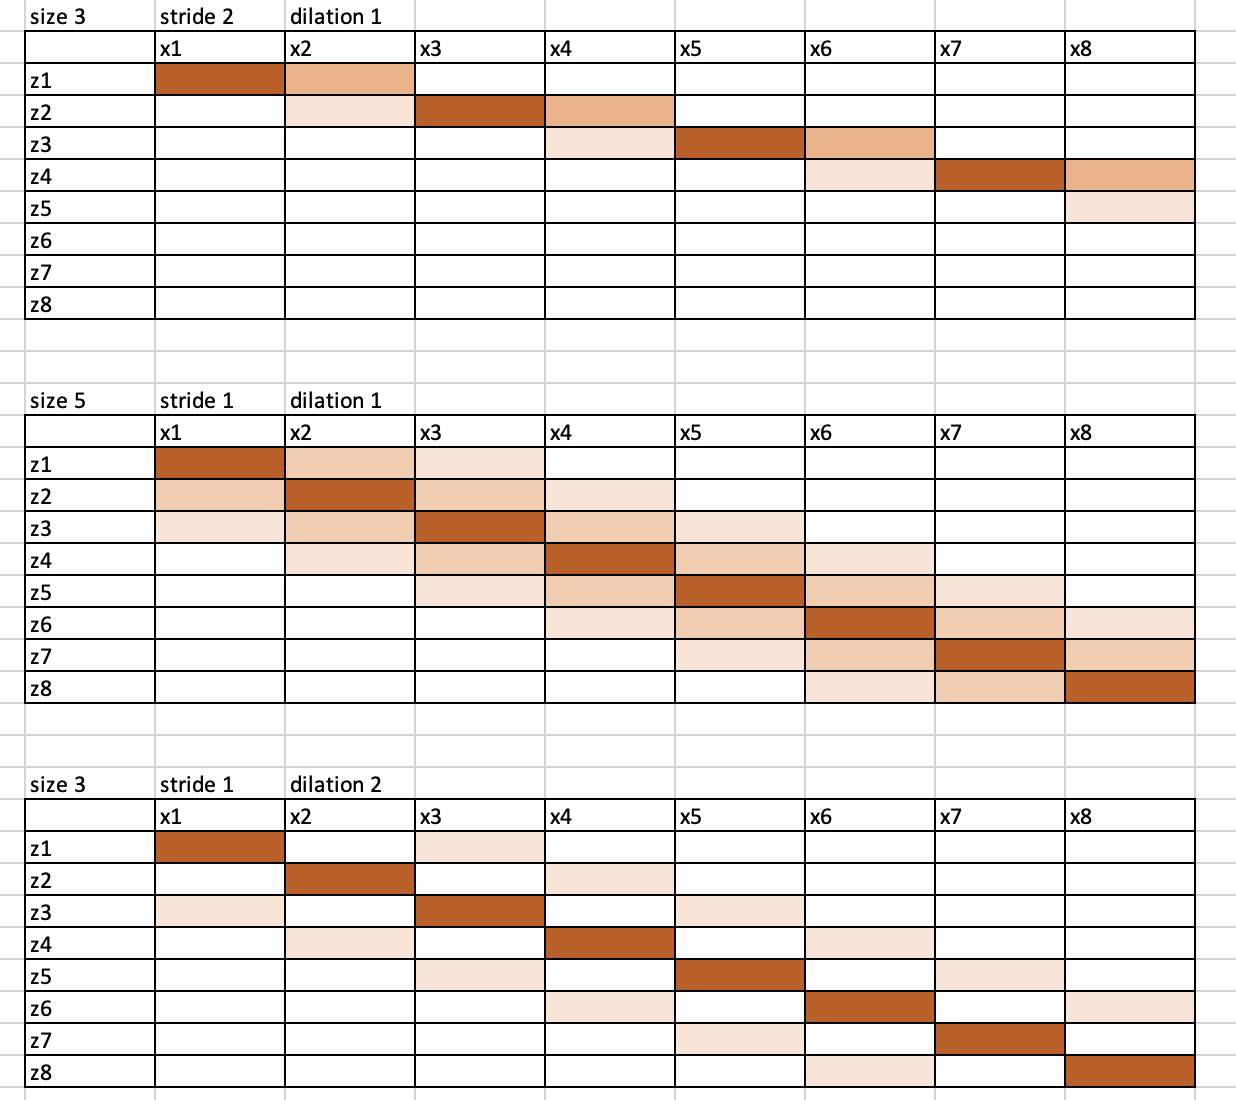
\includegraphics[width=\textwidth]{10_5.png}
    \label{fig:udl_chap10_fig1}
\end{figure}

\subsection{}
\begin{mdframed}
    Draw a $6 \times 12$ weight matrix in the style of figure 10.4d relating the inputs $x_{1}, \dots, x_{6}$ to the outputs $h_{1}, \dots, h_{12}$ in the multi-chanel convolution as depicted in figures 10.5a-b.
\end{mdframed}

\subsection{}
\begin{mdframed}
    Draw a $12 \times 6$ weight matrix in the style of figure 10.4d relating the inputs $h_{1}, \dots, h_{12}$ to the outputs $h_{1}', \dots, h_{6}'$ in the multi-chanel convolution as depicted in figures 10.5c.
\end{mdframed}

\begin{figure}[ht]
    \centering
    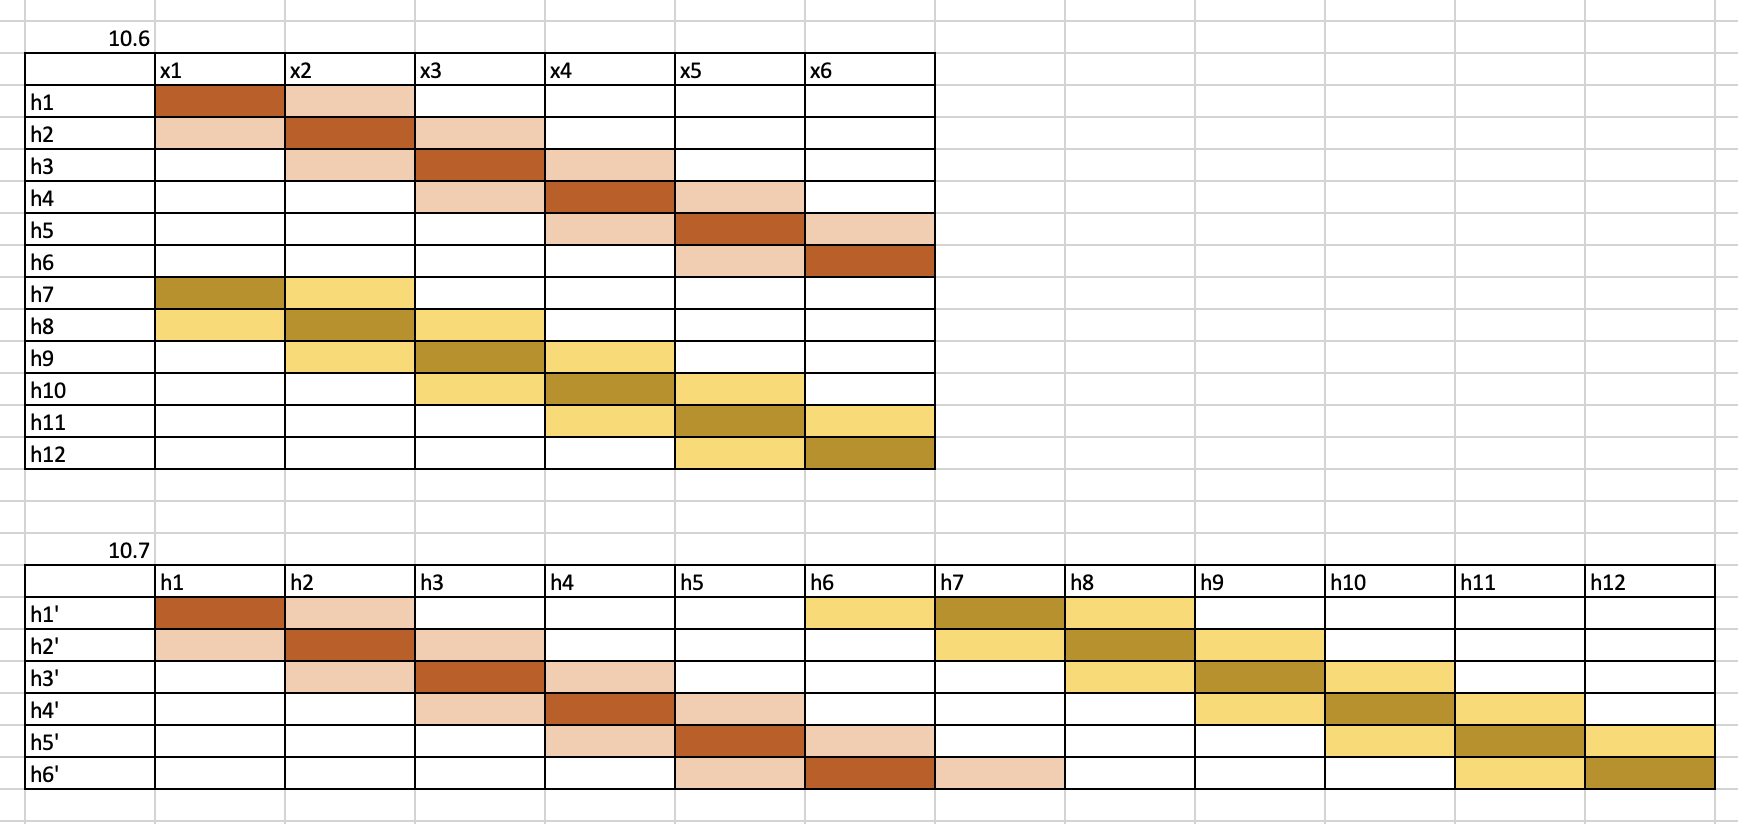
\includegraphics[width=1\textwidth]{10_6_7.png}
    \label{fig:udl_chap10_fig2}
\end{figure}

\subsection{}
\begin{mdframed}
    Consider a 1D convolutional network where the input has three channels. The first hidden layer is computed using a kernel size of three and has four channels. The second hidden layer is computed using a kernel size of five and has ten channels. How many biases and how many weights are needed for each of these two convolutional layers?
\end{mdframed}

For a 1D CNN where the input has three channels, $C_{i} = 3$, the first hidden layer has a kernel size of three and four channels, $K_{1} = 3, C_{1} = 4$, and the second hidden layer has a kernel size of five and ten channels, $K_{2} = 5, C_{2} = 10$, the number of weights and biases for each convolutional layer can be calculated as follows:

For the first layer, there are $3$ input channels, therefore for a single kernel of size $3$ there are $3 \times 3 = 9$ weights, giving a total of $9 \times 4 = 36$ weights. There is one bias per channel, giving a total of $4$ biases.

For the second layer, there are $4$ input channels (from the output size of layer one), therefore a single kernel of size $5$ has $4 \times 5 = 20$ weights, giving a total of $20 \times 10 = 200$ weights in the second layer. There is one bias per output channel, giving a total of $10$ biases.

\newpage

\subsection{}
\begin{mdframed}
    A network consists of three 1D convolutional layers. At each layer, a zero-padded convolution with kernel size three, stride one, and dilation one is applied. What size is the receptive field of the hidden units in the third layer?
\end{mdframed}

Assuming dilation of one means no dilation (as per latest edition of UDL).

The receptive field of layer one is $3$, layer two is $5$, and layer three is $7$.

\subsection{}
\begin{mdframed}
    A network consists of three 1D convolutional layers. At each layer, a zero- padded convolution with kernel size seven, stride one, and dilation one is applied. What size is the receptive field of hidden units in the third layer?
\end{mdframed}

The receptive field of layer one is $7$, layer two is $13$, and layer three is $19$.

\subsection{}
\begin{mdframed}
    Consider a convolutional network with 1D input $\mathbf{x}$. The first hidden layer $\mathbf{H}_{1}$ is computed using a convolution with kernel size five, stride two, and a dilation rate of one. The second hidden layer $\mathbf{H}_{2}$ is computed using a convolution with kernel size three, stride one, and a dilation rate of one. The third hidden layer $\mathbf{H}_{3}$ is computed using a convolution with kernel
    size five, stride one, and a dilation rate of two. What are the receptive field sizes at each hidden layer?
\end{mdframed}

The receptive field of $\mathbf{H}_{1}$ is $5$ ($=$ kernel size).

The receptive field of $\mathbf{H}_{2}$, which has a kernel size of 3 is equal to the receptive field of $\mathbf{H}_{1}$, plus one minus the kernel size of $\mathbf{H}_{2}$, multiplied by the stride of $\mathbf{H}_{1}$: $5 + (3-1) \times 2 = 9$.

If $\mathbf{H}_{3}$ had a dilation of 1, then to calculate the receptive field we would follow the same procedure described above: $9 + (5-1) \times 2 = 17$. However, $\mathbf{H}_{3}$ has a dilation of 2, so we multiply the above equation by 2 again to give $9 + (5-1) \times 2 \times 2 = 25$.


\subsection{}
\begin{mdframed}
    The 1D convolutional network in figure 10.7 was trained using stochastic gradient descent with a learning rate of 0.01 and a batch size of 100 on a training dataset of 4,000 examples for 100,000 steps. How many epochs was the network trained for?
\end{mdframed}

An epoch consists of one full pass through the training dataset. Given the network was trained for 100,000 steps, on 4,000 examples with a batch size of 100, the number of steps per epoch is given by the number of examples divided by the batch size: $4000/100 = 40$. The number of epochs is therefore $100000/40 = 2500$.


\subsection{}
\begin{mdframed}
    Draw a weight matrix in the style of figure 10.4d that shows the relationship between the 24 inputs and the 24 outputs in figure 10.9.
\end{mdframed}

\begin{figure}[ht]
    \centering
    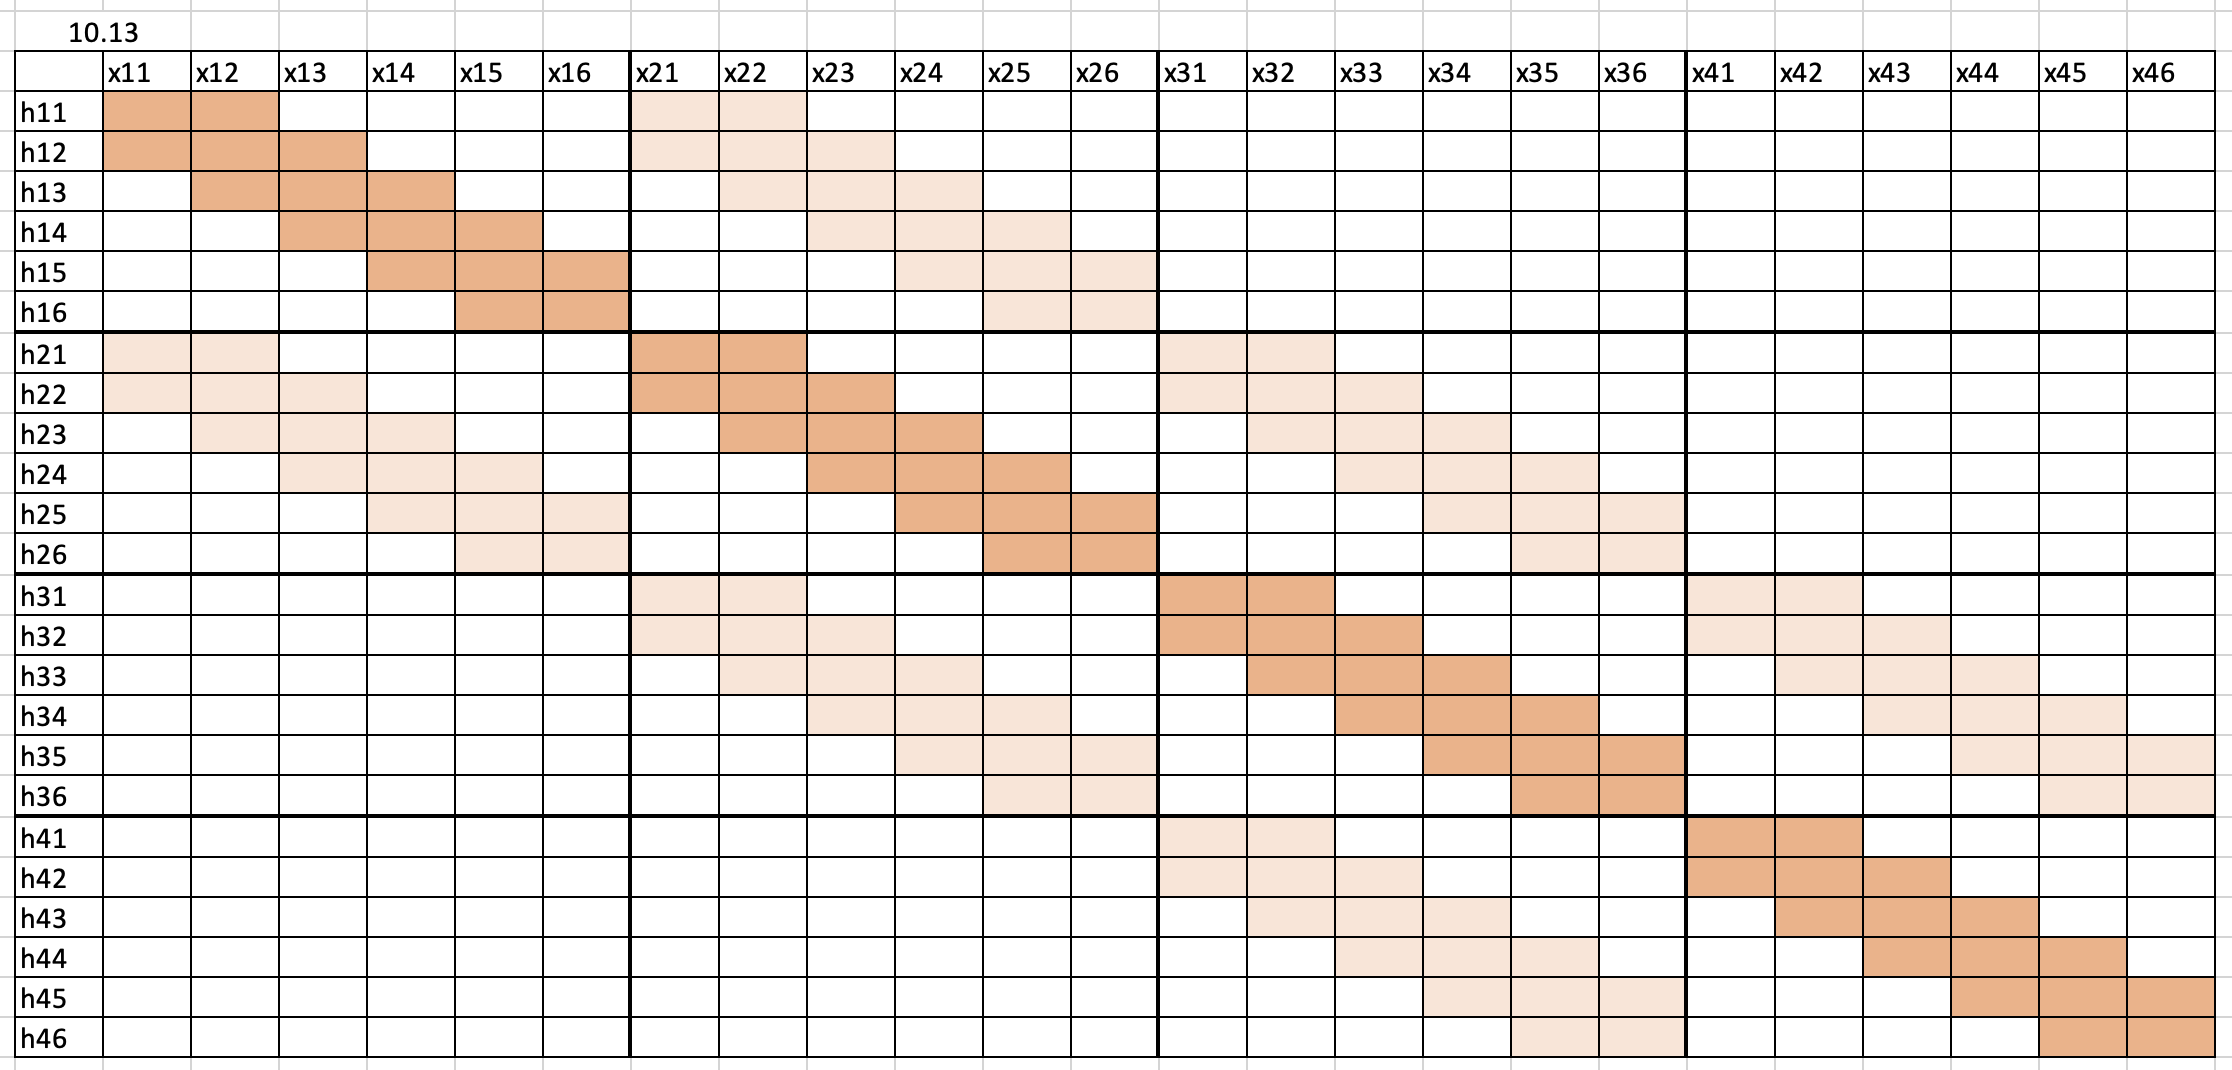
\includegraphics[width=1\textwidth]{10_13.png}
    \label{fig:udl_chap10_fig3}
\end{figure}


\subsection{}
\begin{mdframed}
    Consider a 2D convolutional layer with kernel size $5\times5$ that takes 3 input channels and returns 10 output channels. How many convolutional weights are there? How many biases?
\end{mdframed}

With three input channels, a $5\times5$ kernel would have $5\times5\times3$ weights for one output. Therefore for 10 outputs, there are $5\times5\times3\times10 = 750$ weights. There is one bias per output channel, giving a total of $10$ biases.

\subsection{}
\begin{mdframed}
    Draw a weight matrix in the style of figure 10.4d that samples every other variable in a 1D input (i.e., the 1D analog of figure 10.11a). Show that the weight matrix for 1D convolution with kernel size and stride two is equivalent to composing the matrices for 1D convolution with kernel size one and this sampling matrix.
\end{mdframed}

Unsure about this one...

\subsection{}
\begin{mdframed}
    Consider the AlexNet network (figure 10.16). How many parameters are used in each convolutional and fully connected layer? What is the total number of parameters?
\end{mdframed}

The layers in the AlexNet are as follows:

\begin{itemize}
    \item Conv1: $11\times11$ kernel, 96 output channels, 3 input channels, stride 4. Number of parameters for this layer: $(11\times11\times3+1)\times96 = 34,944$.
    \item Conv2 (+ max pooling): $5\times5$ kernel, 256 output channels, 96 input channels, stride 1. Number of parameters for this layer: $(5\times5\times96+1)\times256 = 614,656$.
    \item Conv3: $3\times3$ kernel, 384 output channels, 256 input channels, stride 1. Number of parameters for this layer: $(3\times3\times256+1)\times384 = 885,120$.
    \item Conv4: $3\times3$ kernel, 384 output channels, 384 input channels, stride 1. Number of parameters for this layer: $(3\times3\times384+1)\times384 = 1,327,488$.
    \item Conv5: $3\times3$ kernel, 256 output channels, 384 input channels, stride 1. Number of parameters for this layer: $(3\times3\times384+1)\times256 = 884,992$.
    \item Max pooling and FC layer 1: 4096 hidden units, input dimensions are $13\times13\times256$. Assuming the maxpooling kernel size is $3\times3$, the output dimensions are $6\times6\times256$. Flattened, this gives $6\times6\times256 = 9216$ input units. Therefore, the parameters for this layer are $(9216+1)\times4096 = 37,752,832$. (+1 accounts for bias)
    \item FC layer 2: 4096 hidden units. Number of parameters = (input + 1) $\times$ output = $(4096+1)\times4096 = 16,781,312$.
    \item FC layer 3: 1000 hidden units. Number of parameters = (input + 1) $\times$ output = $(4096+1)\times1000 = 4,097,000$.
    \item Output layer: 1000 classes
\end{itemize}

Therefore, for AlexNet, the total number of parameters is $34,944 + 614,656 + 885,120 + 1,327,488 + 884,992 + 37,752,832 + 16,781,312 + 4,097,000 = 61,788,344$. (assuming a maxpooling kernel size of $3\times3$ between Conv5 and FC1 layers).

\subsection{}
\begin{mdframed}
    What is the receptive field size at each of the first three layers of AlexNet (figure 10.16)?
\end{mdframed}

The first layer (Conv1) has a kernel size of $11\times11$ and a stride of $4$, the receptive field size is therefore $11$. Assuming the maxpooling kernel is $3\times3$ and stride is 1, the receptive field is $11 + (3-1) \times 4 = 19$. For Conv2, the receptive field is $19 + (5-1) \times 1 = 35$ (as the kernel size for this layer is $5\times5$). For Conv3, the receptive field is $35 + (3-1) \times 4 = 43$.

\subsection{}
\begin{mdframed}
    How many weights and biases are there at each convolutional layer and fully connected layer in the VGG architecture (figure 10.17)?
\end{mdframed}

Skipped.

\subsection{}
\begin{mdframed}
    Consider two hidden layers of size $224\times224$ with C1 and C2 channels, respectively, connected by a $3\times3$ convolutional layer. Describe how to initialize the weights using He initialization.
\end{mdframed}

He initialisation sets the weights of the network from a normal distribution with a mean of 0 and a variance of $\frac{2}{D_{h}}$, where $D_{h}$ is the dimension of the original layer to which the weights were applied. This choice of variance in He initialisation ensures that the weights are scaled in such a way as to not diminish or blow up the gradients during forward and backward propagation.

$D_{h}$ for the first layer is $3\times3\times C_{1}$, and for the second layer is $3\times3\times C_{2}$. Therefore, the weights for the convolutional layer are initialised from a normal distribution with a mean of 0 and a variance of $\frac{2}{3\times3\times C_{1}}$. Similarly, for the second layer, the weights are initialised from a normal distribution with a mean of 0 and a variance of $\frac{2}{3\times3\times C_{2}}$.

\end{document}